\documentclass[11pt, a4paper]{article}

\usepackage{amsmath}
\usepackage{amsfonts} %Matheschriften
\usepackage{amssymb} %Mathesymbole
%\usepackage{mathptmx} % Einstellung für Schriften und Sonderzeichen in mathematischen Umgebungen
                        % ändert SChriftfont
\usepackage{wasysym} % Stellt diverse Sonderzeichen bereit
\usepackage{siunitx}
\usepackage{float}
\usepackage{microtype}
\usepackage{graphicx}
\usepackage{hyperref}
\usepackage{xcolor}
\usepackage[section]{placeins}
% allows for temporary adjustment of side margins
\usepackage{changepage}
\usepackage{rotating}


\usepackage[ngerman]{babel}
\addto\captionsngerman{%
 \renewcommand{\abstractname}{Einleitung}}

\title{Versuch 5: Franz Herz Versuch}
\author{Team 4-11: Jascha Fricker, Benedict Brouwer}

\DeclareSIUnit\electron{e}

\begin{document}
    \maketitle

    \tableofcontents

    \newpage

    \section{Einleitung}
    Der Franck-Hertz-Versuch ist ein wichtiger Versuch in der Atomphysik, der von James Franck und Gustav Hertz durchgeführt wurde1. Der Versuch belegt die Existenz von diskreten Energieniveaus in Atomen und stützt das bohrsche Atommodell. Die Experimente wurden 1914 veröffentlicht und 1922 mit dem Nobelpreis für Physik ausgezeichnet.

    \section{Theorie}

    Die Elektronen beschleunigten können gebundene Elektronen im Gas in höheren Bahnen haben. Die Bahnen sind durch den Bahndrehimpuls
    \begin{equation}
        L = \hbar n
    \end{equation}
    gequantelt. Wenn die Elektronen wieder in ihre ursprünglichen Bahnen zurückfallen, dann werden Photonen mit der Frequenz
    \begin{equation}
        h \cdot f = E_1 - E_2 = h \cdot \frac{c}{\lambda} \label{eq:energie}
    \end{equation}
    freigesetzt. Die Energieniveaus der zwei Gase Hg und Neon sind in den Abbildungen \ref{fig:Hgenergie} und \ref{fig:Neonenergie} dargestellt.

    \begin{figure}[h]
        \centering
        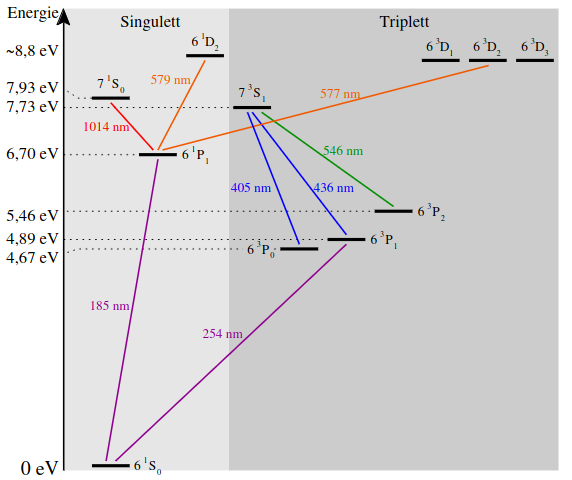
\includegraphics[width=0.5\textwidth]{Screenshot_20230320_160508.png}
        \caption{Energieniveaus von Hg \cite{FHV}}
        \label{fig:Hgenergie}
    \end{figure}

    \begin{figure}[h]
        \centering
        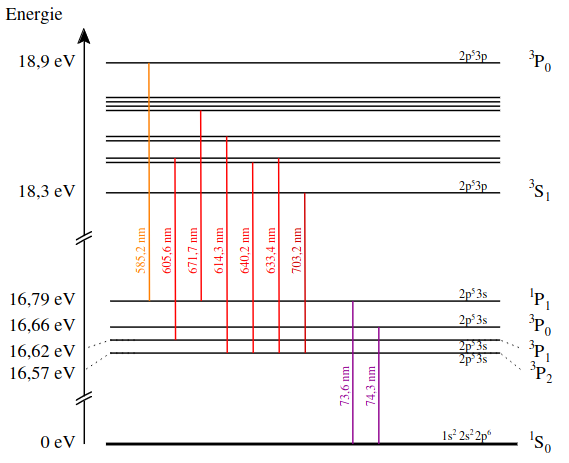
\includegraphics[width=0.5\textwidth]{Screenshot_20230320_160547.png}
        \caption{Energieniveaus von Neon \cite{FHV}}
        \label{fig:Neonenergie}
    \end{figure}

    \section{Versuchsaufbau und Durchführung}

    Der Versuchsaufbau ist in Abbildung \ref{fig:Versuchsaufbau} gezeigt und besteht aus einer Röhre die mit dem jeweilligen Stoff gefüllt ist. Bei Queckssilber muss diese durch einen Ofen erhitzt werden, damit das Quecksilber gasförmig wird. Zwischen der Anode und Kathode wird eine Spannung angelegt, um die Elektronen zu breschleunigen. Mit dem Betriebsgerät wird auch eine kleine negative Spannung an die Auffangelektrode angelegt und dann gemessen, wie viele Elektronen auf die Auffangelektrode treffen, indem der Strom gemessen wird. Durch diesen Auffängerstrom abhängig vom der Beschleunigungsspannung zu beobachten, können dann Rückschlüsse auf die Vorgänge in der Röhre gezogen werden.

    \begin{figure}[h]
        \centering
        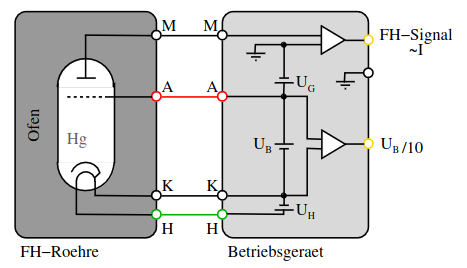
\includegraphics[width=0.5\textwidth]{Screenshot_20230320_160645.png}
        \caption{Versuchsaufbau Hg \cite{FHV}}
        \label{fig:Versuchsaufbau}
    \end{figure}

    \section{Ergebnisse}

    \subsection{Queckssilber}

    Der Gewichtete Mittelwert der Spannungsdifferenzen der Maxima bzw Minima beträgt $E = 4,93(28) \si{\electron\volt}$. Daraus lässt sich eine Wellenlänge von 
    \begin{equation}
        \lambda = \frac{h \cdot c}{E} = 252(14) \si{\nano\meter}
    \end{equation}
    berechnen. Dies passt genau mit dem Übergang von $6^3\text{P}_1$ zu $6^1\text{S}_0$ mit $254 \si{\nano\meter}$ \ref{fig:Hgenergie} überein.
    Die Unsicherheit der Spannung wurde mithilfe der Tabelle 4 des ABW-Skripts \cite{ABW} berechnet. Als Bremsspannung wurde $U_B = 1,72 \si{\volt}$ und als Heizspannung $U_H = 9,51 \si{\volt}$ verwendet.

    \subsection{Neon}

    Der Gewichtete Mittelwert der Spannungsdifferenzen der Maxima bzw Minima beträgt $E = 20,2(11) \si{\electron\volt}$. Daraus lässt sich eine theoretische Wellenlänge von $61,5(35) \si{\nano\meter}$ berechnen. Diese wird aber nicht in einem mal ausgesandt, sondern in mehreren Linien. Die Energie weicht etwas vom Literaturwert von 18,3 eV und 18,9 eV ab \cite{FHV}. Das liegt wahrscheinlich an der sehr begrenzten Anzahl an Messungen.
    Als Bremsspannung wurde $U_B = 8,67 \si{\volt}$ und als Heizspannung $U_H = 4,35 \si{\volt}$ verwendet.
    Mit dem Spektrometer konnten Linien bei $590 \si{\nano\meter}$, $620 \si{\nano\meter}$ und $650 \si{\nano\meter}$ gemessen werden. Infrage kommen die Spektrallinien bei $585,2 \si{\nano\meter}$, $614,3 \si{\nano\meter}$ und $640,2 \si{\nano\meter}$ aus der Abbildung \ref{fig:Neonenergie}.
<<<<<<< HEAD
<<<<<<< HEAD
<<<<<<< HEAD
<<<<<<< HEAD
<<<<<<< HEAD
<<<<<<< HEAD
<<<<<<< HEAD
<<<<<<< HEAD
=======
=======
>>>>>>> dd3207a3d1e46b93caf2deece399e29e43d9c3b2
=======
>>>>>>> d226d60144362f0d14f449bf1baed4029f3ca498
=======
>>>>>>> 9d62b6515dca909649faa05cf46eaf2aa60e580b
=======
>>>>>>> 9d62b6515dca909649faa05cf46eaf2aa60e580b
=======
>>>>>>> 9d62b6515dca909649faa05cf46eaf2aa60e580b
=======
>>>>>>> c1db1765f39811d14f28b3cde6b5e69e0118b8ab
=======
>>>>>>> c1db1765f39811d14f28b3cde6b5e69e0118b8ab

    \section{Fragen}

    \begin{enumerate}
        \item Ein elastischer Stoß ist ein Stoß, bei dem die kinetische Energie und der Impuls erhalten bleiben. Das bedeutet, dass die Gesamtenergie und der Gesamtimpuls des Systems vor und nach dem Stoß gleich sind.

        Ein inelastischer Stoß ist ein Stoß, bei dem die kinetische Energie nicht erhalten bleibt. Dabei Stoßen zwei Teilchen zusammen und werden zu einem. Ein Teil der kinetischen Energie wird in innere Energie umgewandelt. Das bedeutet, dass die kinetische Energie des Systems nach dem Stoß kleiner ist als die kinetische Energie des Systems vor dem Stoß.

        \item Ein Elektron mit einer Energie von weniger als 4,9 eV kann nur einen elastischen Stoß mit einem Atom machen, weil es nicht genügend Energie hat, um die nächste gequantelte Bahn zu "erreichen" und somit seine Energie an das Atom abzugeben.
        \item Da das Atom viel schwer ist, ist es etwa so, wie wenn das Elektron gegen ein festes Objekt "stoßen" würde. Das Elektron behält also fast die gesamte Energie.
        \item Das angeregte Atom emittiert ein Photon, wenn ein Elektron in eine niedrigere Bahn fällt. So gibt es die Energie ab. Dies kann mehrmals hintereinander passieren, bis das Elektron in der niedrigsten möglichen Bahn ist. Dann ist das Atom wieder in seinem Grundzustand.
        \item Das Photon muss genau eine der Anregunsenergieen des Atoms haben, um dieses anzuregen. Das Elektron hingegen kann auch nur einen Teil der Energie an das Atom abgeben.
        \item Die Bremsspannung lässt nur Elektronen mit höherer Geschwindigkeit durch, die Ausreichend ist, um das Elektrische Feld zu überwinden, und wirkt damit als Geschwindigkeits-Filter. Nur so enststehen die Maxima und Minima beim Strom.
        \item Das Funktionsprinzip einer Frank-Herz Röhre unterscheidet sich ein wenig von der einer Leuchtstoffröhre. Bei beiden werden aus einer Grühkathode ausgelößte Elektronen durch ein Elektrisches Feld beschleunigt. Während bei der Frank-Herz Röhre die Atome nur angeregt werden, werden sie in einer Leuchtstoffröhre zu einem Plasma ionisiert. Durch den Leuchstoff an den Außenwänden werdir die UV-Strahlung des Quecksilbers in sichtbares Licht umgewandelt. Der Starten lässt beim Einschaltvorgang Strom durch die Glühwendel fließen, um sie aufzuheizen. Wenn die Röhre Leuchtet und sie durch Ionenbombardement auf Temperatur gehalten werden, ist dies nicht mehr nötig. Die Drosselspuhle begrenzt den durchs Plasma fließend Strom, die Leuchtstoffröhre wird im gegensaatz zur Frank-Herz Röhre mit einer Wechselspannung betrieben, weshalb die Kathode und Anode ständig wechseln.
        \item Eine Röntgenröhre ist mit Vakuum gefüllt und die Strahlung wird durch Bremsstrahlung und den Photoeffekt erzeugt. Bei Frankherzversuch wird die Strahlung durch die angergen Atome erzeugt, außerdem sind die Wellenlängen viel länger, da die Atome nicht ionisiert werden. 
        
        
    \end{enumerate}

        

<<<<<<< HEAD
<<<<<<< HEAD
<<<<<<< HEAD
<<<<<<< HEAD
<<<<<<< HEAD
<<<<<<< HEAD
<<<<<<< HEAD
>>>>>>> dd3207a3d1e46b93caf2deece399e29e43d9c3b2
=======
>>>>>>> dd3207a3d1e46b93caf2deece399e29e43d9c3b2
=======
>>>>>>> d226d60144362f0d14f449bf1baed4029f3ca498
=======
>>>>>>> 9d62b6515dca909649faa05cf46eaf2aa60e580b
=======
>>>>>>> 9d62b6515dca909649faa05cf46eaf2aa60e580b
=======
>>>>>>> 9d62b6515dca909649faa05cf46eaf2aa60e580b
=======
>>>>>>> c1db1765f39811d14f28b3cde6b5e69e0118b8ab
=======
>>>>>>> c1db1765f39811d14f28b3cde6b5e69e0118b8ab
    \bibliographystyle{plain}
    \bibliography{literature}

\end{document}